\documentclass[11pt,letterpaper]{article}

% ---------------------------------------------------------------------------
% Portable font & encoding setup (works with pdflatex, xelatex, lualatex, tectonic)
% ---------------------------------------------------------------------------
\usepackage{iftex}
\ifPDFTeX
  \usepackage[utf8]{inputenc}
\fi
\usepackage[T1]{fontenc}
\usepackage{mathpazo}
\usepackage[scaled=0.92]{helvet}
\usepackage{courier}

% ---------------------------------------------------------------------------
% Page layout, typography, math, tables, graphics, TikZ, citations
% ---------------------------------------------------------------------------
\usepackage[margin=1.0in,headheight=16pt]{geometry}
\usepackage{microtype}
\usepackage{amsmath,amssymb}
\usepackage{graphicx}
\usepackage{booktabs}
\usepackage{array}
\usepackage{tabularx}
\usepackage{multirow}
\usepackage{enumitem}
\usepackage{xcolor}
\usepackage{colortbl}
\usepackage[font=small,labelfont=bf,labelsep=period,skip=6pt]{caption}
\usepackage{subcaption}
\usepackage{fancyhdr}
\usepackage{titlesec}
\usepackage{natbib}
\usepackage{xurl}
\usepackage{tikz}
\usetikzlibrary{arrows.meta,positioning,shapes.geometric,patterns,calc}
\usepackage[hidelinks,colorlinks=true,linkcolor=accentBlue,citecolor=accentBlue,urlcolor=accentBlue]{hyperref}

% Generous float parameters so tables and figures stay near their text references
\renewcommand{\topfraction}{0.90}
\renewcommand{\bottomfraction}{0.80}
\renewcommand{\textfraction}{0.08}
\renewcommand{\floatpagefraction}{0.75}
\setcounter{topnumber}{3}
\setcounter{bottomnumber}{2}
\setcounter{totalnumber}{4}

% ---------------------------------------------------------------------------
% Palette (aligned with the benchmark figures)
% ---------------------------------------------------------------------------
\definecolor{accentBlue}{HTML}{006699}
\definecolor{cmykC}{HTML}{00A0D6}
\definecolor{cmykCDeep}{HTML}{0081AD}
\definecolor{cmykCTint}{HTML}{E3F5FB}
\definecolor{cmykCMid}{HTML}{7FCFEA}
\definecolor{cmykM}{HTML}{E0218A}
\definecolor{cmykMDeep}{HTML}{B8156E}
\definecolor{cmykMTint}{HTML}{FDE6F1}
\definecolor{cmykMMid}{HTML}{F09BC8}
\definecolor{neonBlue}{HTML}{2F55C4}
\definecolor{neonTint}{HTML}{E8EEFC}
\definecolor{neonMid}{HTML}{7F9AE0}
\definecolor{oppOrange}{HTML}{E05A2B}
\definecolor{inkDark}{HTML}{111111}
\definecolor{inkMuted}{HTML}{666660}
\definecolor{ruleGrey}{HTML}{D4D4CE}
\definecolor{fogGrey}{HTML}{EAEAE5}
\definecolor{winTint}{HTML}{EFF5FC}
\definecolor{headerBg}{HTML}{F5F6F8}

% ---------------------------------------------------------------------------
% Section styling & running header
% ---------------------------------------------------------------------------
\titleformat{\section}{\large\bfseries\sffamily}{\thesection}{0.75em}{}
\titleformat{\subsection}{\normalsize\bfseries\sffamily}{\thesubsection}{0.65em}{}
\titlespacing*{\section}{0pt}{14pt plus 3pt minus 2pt}{5pt plus 1pt}
\titlespacing*{\subsection}{0pt}{10pt plus 2pt minus 2pt}{4pt plus 1pt}

\pagestyle{fancy}
\fancyhf{}
\renewcommand{\headrulewidth}{0.4pt}
\renewcommand{\headrule}{\hbox to\headwidth{\color{ruleGrey}\leaders\hrule height \headrulewidth\hfill}}
\fancyhead[L]{\footnotesize\sffamily\color{inkMuted} VibeResearch Bench}
\fancyhead[R]{\footnotesize\sffamily\color{inkMuted} Zhang \& Bittker}
\fancyfoot[C]{\footnotesize\sffamily\color{inkMuted}\thepage}

\fancypagestyle{firstpage}{
  \fancyhf{}
  \renewcommand{\headrulewidth}{0pt}
  \fancyfoot[C]{\footnotesize\sffamily\color{inkMuted}\thepage}
}

\setlist[itemize]{leftmargin=1.4em,itemsep=3pt,topsep=4pt}
\renewcommand{\arraystretch}{1.16}

% Handy commands
\newcommand{\pokemon}{Pok\'emon}
\newcommand{\mult}[1]{\ensuremath{#1\times}}

% ---------------------------------------------------------------------------
% Document
% ---------------------------------------------------------------------------
\begin{document}
\thispagestyle{firstpage}

% --- Preprint-style Title Block ---
\begin{center}
  \rule{\linewidth}{1.6pt}\\[10pt]
  {\LARGE\bfseries\sffamily VibeResearch Bench:\\[3pt]
  Can AI Agents Train Strong Game Bots on a Budget?\par}
  \vspace{8pt}
  \rule{\linewidth}{0.5pt}\\[12pt]
  {\normalsize\bfseries
    \href{https://x.com/kzdagoof}{Kevin Zhang} \qquad
    \href{https://x.com/maxbittker}{Max Bittker}
  }\\[5pt]
  {\small\color{inkMuted}
    November 19, 2026 \quad$\cdot$\quad
    Interactive results, replays, and code: \url{https://gameautoresearch.github.io/}
  }
\end{center}
\vspace{6pt}

% --- Abstract ---
\begin{abstract}
\noindent
AI agents have demonstrated superhuman proficiency at writing deterministic software, yet machine learning research poses fundamentally different challenges: allocating finite compute budgets, designing informative experiments, and reasoning under noisy training signals. We introduce \textbf{VibeResearch Bench}, a benchmark evaluating how effectively frontier AI agents can autonomously train efficient domain-specific reinforcement learning (RL) policies on a fixed GPU budget across three strategic game environments: \pokemon{} 3v3, \textit{The Battle of Polytopia}, and \textit{Generals.io}. Across five benchmark tasks---including training from an empty file, improving a working RL starter under varying dollar budgets, engineering faster simulators, forecasting run outcomes prior to spending compute, and competing in a 20-network tournament---we evaluate ten frontier models using a unified agent harness on NVIDIA L40S GPUs. We observe wide separation in research taste, compute efficiency, and final policy strength. \textbf{Gemini 4 Neon} ranks first overall ($58.5 \pm 1.2$ on a standardized 50-mean, 10-SD scale), followed by \textbf{Claude Fable 5.2} ($55.9 \pm 2.3$) and \textbf{Gemini 4 Carbon} ($54.1 \pm 3.4$). While most researched training recipes fail to recoup their research spend within 8~hours of downstream training, standout sessions achieve dramatic returns: a single \$8.58 Polytopia session by Gemini 4 Neon trains an 8-hour policy matching roughly 108~hours (\$313) of baseline starter training---about \mult{10} less total compute (and \mult{12.8} training-only efficiency). Case studies reveal that stronger research agents run disciplined, short A/B experiments, rebuild slow Python simulators in batched JAX (achieving up to \mult{25} throughput gains), and outperform regression baselines when forecasting run outcomes before launch. Finally, evaluating 30 models released between February and November 2026 documents a rapid capability transition: models progressed from failing to beat random play in early 2026 to surpassing a tuned PPO baseline on the same compute budget by autumn 2026.
\end{abstract}

% ===========================================================================
\section{Introduction}
\label{sec:intro}

Can AI agents train strong domain-specific models? AI coding agents have already demonstrated superhuman skills when writing deterministic code. However, machine learning research imposes a distinct set of demands: operating under limited compute, contending with stochastic and noisy training signals, deciding which hypotheses merit investment, and knowing when an experimental result is strong enough to justify committing the remainder of a budget.

To study these capabilities systematically, we gave frontier AI models a fixed GPU budget and tasked them with training efficient neural networks to play complex strategy games: \pokemon{} (3v3 Random Battle), \textit{The Battle of Polytopia}, and \textit{Generals.io}. Within isolated workspaces, agents allocated their own compute, implemented architectural and algorithmic ideas, ran evaluations, and iterated to produce the strongest final policies. Across models, we observed substantial variation in research taste, experimental efficiency, and final policy strength.

Just as ``vibe-coding'' has led to a proliferation of custom software, ``vibe-training'' promises new frontiers of specialized neural networks tailored to niche domains. Yet the practical efficiency of such agent-driven workflows depends critically on the agent's research judgment: carefully measuring progress, selecting high-leverage interventions, and allocating limited training runs. Throughout our evaluations, stronger agents consistently trained markedly stronger policies for smaller budgets. Table~\ref{tab:showcase} illustrates representative agent-trained policies across all three featured game domains, showing the diversity of architectures, throughput optimizations, and RL recipes discovered autonomously under modest L40S budgets.

\begin{table}[htbp]
\centering
\caption{Representative RL policies autonomously trained by AI agents across the three featured game environments on NVIDIA L40S GPUs (\$2.903/GPU-hour). \pokemon{} 3v3 entries reflect fresh $\sim$55-minute final retrains; Polytopia entries reflect 2-hour recipe finals (plus GPT-6 Astra's refined policy and the 200M-sample baseline); Generals.io entries reflect the slow-simulator campaign (cumulative training GPU time and achieved simulation throughput).}
\label{tab:showcase}
\scriptsize
\renewcommand{\arraystretch}{1.10}
\setlength{\tabcolsep}{4pt}
\begin{tabularx}{\textwidth}{@{}llrr>{\raggedright\arraybackslash}p{3.65cm}>{\raggedright\arraybackslash}X@{}}
\toprule
\textbf{Game} & \textbf{Agent / Policy} & \textbf{Size / Speed} & \textbf{GPU (Cost)} & \textbf{Architecture / Engine} & \textbf{Training Regime} \\
\midrule
\multirow{5}{*}{\pokemon{} 3v3}
  & GPT-6.1 Sol (a1)     & 338K params & 0.93\,h (\$2.70) & 96w MLP; damage, STAB \& Tera prior & PPO (2 ep, $\gamma{=}0.997$) + HP shaping \\
  & GPT-6 Astra (a1)     & 477K params & 0.93\,h (\$2.70) & 128w MLP; stat-stage combat head & PPO (3 ep, $\gamma{=}0.995$) + HP shaping \\
  & Inkling 2 Small (b2) & 526K params & 0.93\,h (\$2.70) & 2$\times$ wider starter MLP (128w, 16d emb) & Self-play PPO, 2$\times$ entropy (0.02) \\
  & DeepSeek V4 Pro (a2) & 814K params & 0.93\,h (\$2.70) & 2-layer SiLU MLPs (160w, 20d emb) & PPO + $0.5\times$ team-HP shaping \\
  & GLM-5.3 (a3)         & 903K params & 0.93\,h (\$2.70) & 320w side-aware cross-attention & Plain self-play PPO, unshaped \\
\midrule
\multirow{4}{*}{Polytopia}
  & Claude Opus 5.5      & 192K params & 2.0\,h (\$5.72)  & $2{\times}32$ ResNet + autoregressive heads & 2-ep PPO, LR decay + score bonus \\
  & GPT-6 Astra (ref.)   & 390K params & 2.7\,h (\$10.36) & $3{\times}48$ context-v3 ResNet (global$\to$tile) & Score shaping + low-LR refine \\
  & GPT-6.1 Sol          & 192K params & 2.0\,h (\$5.71)  & $2{\times}32$ ResNet + autoregressive heads & Self-play PPO, $\gamma{=}1.0$ + dev reward \\
  & Starter (200M)       & 192K params & $\sim$0.7\,h (\$2.00) & $2{\times}32$ ResNet + autoregressive heads & Plain self-play PPO (200M samples) \\
\midrule
\multirow{4}{*}{Generals.io}
  & Claude Opus 5.5      & $\sim$14.6k/s & 2.7\,h (\$7.73) & Rebuilt batched JAX sim + jitted PPO & 7 chained runs, anchored self-play \\
  & GPT-6.1 Sol          & $\sim$5.4k/s  & 3.3\,h (\$11.23) & Rebuilt batched JAX sim (37M ticks) & PPO + shaping, pool \& symmetries \\
  & Kimi K3.1 Pro        & $\sim$630/s   & 2.4\,h (\$7.11)  & $5{\times}64$ ResNet on supplied Python sim & PPO + reward tuning ($\sim$5M ticks) \\
  & DeepSeek V4 Pro      & $\sim$565/s   & 2.3\,h (\$6.57)  & $8{\times}96$ CNN on supplied Python sim & PPO + castle rewards ($\sim$5M ticks) \\
\bottomrule
\end{tabularx}
\end{table}

% ===========================================================================
\section{Benchmark Design}
\label{sec:design}

We designed VibeResearch Bench so that agents must manage the research lifecycle like an autonomous ML researcher: deciding which ideas are worth testing, how long each experiment should run, and when a practice evaluation is convincing enough to justify betting the remaining compute budget. Every research session runs inside a uniform sandboxed workspace driven by Harbor's Terminus-2 harness, where each agent receives:

\begin{itemize}
  \item \textbf{Compute on Modal.} A fixed GPU dollar or hour budget together with a command-line interface to launch training jobs on NVIDIA L40S workers (\$2.903/GPU-hour) and inspect logs. All allocated worker time---including compilation, simulation, training, checkpointing, and failed jobs---counts against the budget.
  \item \textbf{A game rulebook.} An offline reference describing the game rules, entity mechanics, legal actions, observation schemas, and exact scoring definitions.
  \item \textbf{A simulator.} Most tasks provide an optimized game simulator (e.g., JAX/GPU or native engines). In one Generals.io variant, agents instead receive an accurate but slow, single-threaded Python simulator that they are free to profile and rewrite.
  \item \textbf{Editable training code and configurations.} Depending on the task, agents begin either from a deliberately minimal working PPO starter or from an empty training scaffold containing no learning code.
  \item \textbf{A practice evaluation suite.} Agents can evaluate intermediate checkpoints against fixed public practice opponents during their session to guide iteration and final submission selection. Official grading uses held-out private evaluation panels, seeds, or multi-agent tournaments.
\end{itemize}

\subsection{Submission Formats}

Each benchmark task uses one of two submission formats, illustrated in Figure~\ref{fig:formats}:
\begin{enumerate}[leftmargin=1.5em,itemsep=2pt]
  \item \textbf{Submit a trained model (\texttt{network} variant).} The agent trains the final policy network itself and submits the serialized weights directly for evaluation. Exploratory tests and the final training run draw from the same compute budget, forcing an explicit exploration--exploitation trade-off.
  \item \textbf{Submit a training recipe (\texttt{recipe} variant).} The agent spends its entire research budget on diagnostic experiments and submits training code plus hyperparameters. The benchmark harness then executes a fresh retrain from scratch on a separate, fixed compute budget before grading.
\end{enumerate}

\begin{figure}[t]
\centering
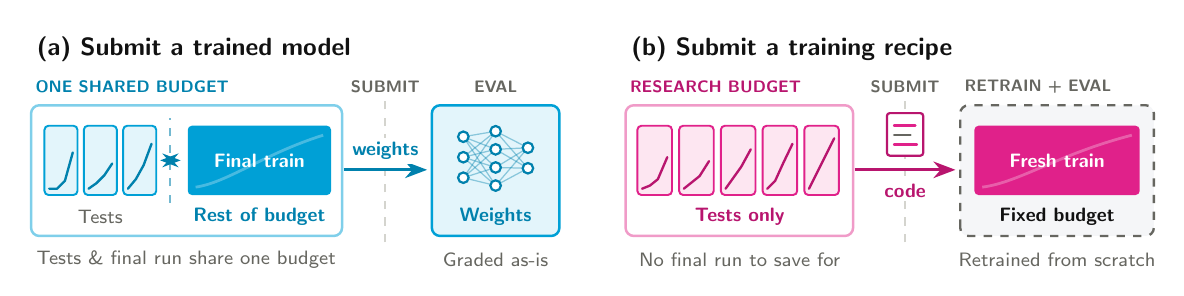
\begin{tikzpicture}[
  font=\sffamily,
  >=Stealth,
  kicker/.style={font=\sffamily\bfseries\fontsize{6.5}{7.5}\selectfont, inner sep=0pt},
  sub/.style={font=\sffamily\fontsize{7.0}{8.0}\selectfont, inner sep=0pt},
  fcap/.style={font=\sffamily\fontsize{6.8}{7.8}\selectfont, text=inkMuted, inner sep=0pt}
]

% ================= LEFT PANEL: SUBMIT A TRAINED MODEL =================
\begin{scope}[shift={(0,0)}]
  \node[anchor=west, font=\sffamily\bfseries\small, text=inkDark] at (0, 2.75) {(a) Submit a trained model};

  % Headers
  \node[kicker, anchor=west, text=cmykCDeep] at (0.1, 2.28) {ONE SHARED BUDGET};
  \node[kicker, text=inkMuted] at (4.55, 2.28) {SUBMIT};
  \node[kicker, text=inkMuted] at (5.95, 2.28) {EVAL};

  % Submission boundary
  \draw[ruleGrey, dashed, line width=0.7pt] (4.55, 0.30) -- (4.55, 2.12);

  % Shared budget container
  \draw[cmykCMid, line width=0.9pt, rounded corners=3pt, fill=white] (0.05, 0.38) rectangle (4.00, 2.04);

  % Three short probes
  \foreach \px/\ya/\yb/\yc in {0.22/0.98/1.08/1.44, 0.72/1.05/1.15/1.30, 1.22/1.10/1.28/1.55} {
    \draw[cmykC, fill=cmykCTint, rounded corners=1.5pt, line width=0.7pt] (\px, 0.90) rectangle (\px+0.42, 1.78);
    \draw[cmykCDeep, line width=0.85pt, line cap=round, line join=round]
      (\px+0.06, 0.98) -- (\px+0.16, \ya) -- (\px+0.26, \yb) -- (\px+0.36, \yc);
  }

  % Tradeoff divider
  \draw[cmykCDeep, dashed, opacity=0.55, line width=0.7pt] (1.82, 0.80) -- (1.82, 1.88);
  \draw[cmykCDeep, line width=0.8pt, <->] (1.69, 1.34) -- (1.95, 1.34);

  % Final training run block
  \fill[cmykC, rounded corners=1.5pt] (2.04, 0.90) rectangle (3.86, 1.78);
  \draw[white, opacity=0.28, line width=1.0pt] (2.14, 1.00) .. controls (2.55, 1.06) and (3.00, 1.42) .. (3.76, 1.66);
  \node[font=\sffamily\bfseries\fontsize{7.5}{8.5}\selectfont, text=white] at (2.95, 1.34) {Final train};

  % Labels inside container
  \node[sub, text=inkMuted] at (0.93, 0.62) {Tests};
  \node[sub, font=\sffamily\bfseries\fontsize{7.0}{8.0}\selectfont, text=cmykCDeep] at (2.95, 0.62) {Rest of budget};

  % Arrow to eval
  \draw[cmykCDeep, line width=1.1pt, ->] (4.02, 1.22) -- (5.08, 1.22);
  \node[sub, font=\sffamily\bfseries\fontsize{6.8}{7.8}\selectfont, text=cmykCDeep, fill=white, inner sep=1.5pt] at (4.55, 1.46) {weights};

  % Eval card with mini NN
  \draw[cmykC, fill=cmykCTint, rounded corners=3pt, line width=0.9pt] (5.14, 0.38) rectangle (6.76, 2.04);
  \foreach \yone in {1.12, 1.38, 1.64} {
    \foreach \ytwo in {1.02, 1.25, 1.48, 1.71} {
      \draw[cmykCDeep, opacity=0.4, line width=0.45pt] (5.54, \yone) -- (5.95, \ytwo);
    }
  }
  \foreach \ytwo in {1.02, 1.25, 1.48, 1.71} {
    \foreach \ythree in {1.24, 1.50} {
      \draw[cmykCDeep, opacity=0.4, line width=0.45pt] (5.95, \ytwo) -- (6.36, \ythree);
    }
  }
  \foreach \yone in {1.12, 1.38, 1.64} {
    \filldraw[fill=white, draw=cmykCDeep, line width=0.8pt] (5.54, \yone) circle (1.9pt);
  }
  \foreach \ytwo in {1.02, 1.25, 1.48, 1.71} {
    \filldraw[fill=white, draw=cmykCDeep, line width=0.8pt] (5.95, \ytwo) circle (1.9pt);
  }
  \foreach \ythree in {1.24, 1.50} {
    \filldraw[fill=white, draw=cmykCDeep, line width=0.8pt] (6.36, \ythree) circle (1.9pt);
  }
  \node[sub, font=\sffamily\bfseries\fontsize{7.0}{8.0}\selectfont, text=cmykCDeep] at (5.95, 0.62) {Weights};

  % Footers
  \node[fcap] at (2.02, 0.08) {Tests \& final run share one budget};
  \node[fcap] at (5.95, 0.08) {Graded as-is};
\end{scope}

% ================= RIGHT PANEL: SUBMIT A TRAINING RECIPE =================
\begin{scope}[shift={(7.55,0)}]
  \node[anchor=west, font=\sffamily\bfseries\small, text=inkDark] at (0, 2.75) {(b) Submit a training recipe};

  % Headers
  \node[kicker, anchor=west, text=cmykMDeep] at (0.1, 2.28) {RESEARCH BUDGET};
  \node[kicker, text=inkMuted] at (3.60, 2.28) {SUBMIT};
  \node[kicker, anchor=west, text=inkMuted] at (4.35, 2.28) {RETRAIN + EVAL};

  % Submission boundary
  \draw[ruleGrey, dashed, line width=0.7pt] (3.60, 0.30) -- (3.60, 2.12);

  % Research-only container
  \draw[cmykMMid, line width=0.9pt, rounded corners=3pt, fill=white] (0.05, 0.38) rectangle (2.94, 2.04);

  % Five probes filling budget
  \foreach \px/\ya/\yb/\yc in {
    0.20/1.02/1.10/1.38,
    0.73/1.06/1.14/1.33,
    1.26/1.12/1.26/1.48,
    1.79/1.08/1.30/1.55,
    2.32/1.18/1.38/1.62
  } {
    \draw[cmykM, fill=cmykMTint, rounded corners=1.5pt, line width=0.7pt] (\px, 0.90) rectangle (\px+0.44, 1.78);
    \draw[cmykMDeep, line width=0.85pt, line cap=round, line join=round]
      (\px+0.06, 0.98) -- (\px+0.16, \ya) -- (\px+0.26, \yb) -- (\px+0.38, \yc);
  }
  \node[sub, font=\sffamily\bfseries\fontsize{7.0}{8.0}\selectfont, text=cmykMDeep] at (1.50, 0.62) {Tests only};

  % Submission arrow + mini code icon
  \draw[cmykMDeep, line width=1.1pt, ->] (2.96, 1.22) -- (4.24, 1.22);
  % Mini code doc
  \draw[cmykMDeep, fill=white, line width=0.8pt, rounded corners=1pt] (3.37, 1.40) rectangle (3.83, 1.94);
  \draw[cmykM, line width=0.9pt, line cap=round] (3.46, 1.78) -- (3.73, 1.78);
  \draw[inkMuted, line width=0.8pt, line cap=round] (3.46, 1.66) -- (3.67, 1.66);
  \draw[cmykM, line width=0.9pt, line cap=round] (3.46, 1.54) -- (3.75, 1.54);
  \node[sub, font=\sffamily\bfseries\fontsize{6.8}{7.8}\selectfont, text=cmykMDeep, fill=white, inner sep=1.5pt] at (3.60, 0.96) {code};

  % Separate benchmark retrain container
  \draw[inkMuted, dashed, line width=0.85pt, rounded corners=3pt, fill=headerBg] (4.30, 0.38) rectangle (6.76, 2.04);
  \fill[cmykM, rounded corners=1.5pt] (4.48, 0.90) rectangle (6.58, 1.78);
  \draw[white, opacity=0.28, line width=1.0pt] (4.58, 1.00) .. controls (5.05, 1.06) and (5.55, 1.42) .. (6.48, 1.66);
  \node[font=\sffamily\bfseries\fontsize{7.5}{8.5}\selectfont, text=white] at (5.53, 1.34) {Fresh train};
  \node[sub, font=\sffamily\bfseries\fontsize{7.0}{8.0}\selectfont, text=inkDark] at (5.53, 0.62) {Fixed budget};

  % Footers
  \node[fcap] at (1.50, 0.08) {No final run to save for};
  \node[fcap] at (5.53, 0.08) {Retrained from scratch};
\end{scope}

\end{tikzpicture}
\caption{The two submission formats used in VibeResearch Bench. \textbf{(a)}~In the trained-model format, exploratory tests and the final training run draw from one shared budget, and submitted weights are graded directly. \textbf{(b)}~In the training-recipe format, the agent devotes its entire research budget to experimentation and submits code that is retrained from scratch on a separate fixed compute allocation.}
\label{fig:formats}
\end{figure}

\subsection{Task Suite and Evaluation Protocol}
\label{sec:tasks}

We grade ten frontier models across five model-training tasks spanning three games and both submission formats:
\begin{enumerate}[leftmargin=1.5em,itemsep=2pt]
  \item \textbf{Polytopia (empty file):} A 5-GPU-hour autoresearch session starting from an empty training scaffold to produce a 15-minute training recipe on $11{\times}11$ fog-of-war Bardur drylands maps (30-round horizon), evaluated via fresh 15-minute retrains and pooled Bradley--Terry Elo across 2.5~million games.
  \item \textbf{Polytopia (multi-budget recipes):} Improving a working PPO starter across five researched budget/time cells (\$2.90, \$8.70, \$23, and \$8.70 under 2\,h or 4\,h wall-clock limits), evaluated via both 1-hour (two-seed) and 8-hour fresh retrains measured in training-compute multipliers adjusted for cell difficulty (Appendix~\ref{app:scoring}).
  \item \textbf{\pokemon{} 3v3 (working starter):} Improving a working PPO starter for Gen~9 3v3 Random Battle (with switching and Terastallization), scored on a 0--100 scale against three independent retrains of the unmodified starter ($50 = \text{level}$).
  \item \textbf{Forecasting training runs:} Predicting held-out outcomes of 181 anonymized \pokemon{} runs (35 final recipes and 146 intermediate training runs) using only pre-launch evidence (code, recipe configuration, and prior practice results), scored by relative forecast skill ($0 = \text{blind guess}$, $1 = \text{perfect}$).
  \item \textbf{Generals.io (20-network tournament):} Training a policy from an empty starter with an editable slow simulator under a 3-L40S-hour research budget (trained-model format), ranked in a 20-network round-robin tournament (190 pairings, 48,640 games across 128 maps in both seats; Bradley--Terry Elo centered at 1000).
\end{enumerate}

To aggregate heterogeneous task units onto a single comparable scale without retroactive score drift as new models are evaluated, each task is standardized against frozen constants computed over the ten reference models: a score of $50$ equals the reference-group mean and $+10$ points correspond to $+1$ standard deviation (using log-multipliers for the Polytopia recipe ratio task; full constants are detailed in Appendix~\ref{app:scoring}). A model's overall score is the unweighted mean of its five standardized task scores, reported with $\pm 1$ standard error across tasks.

% ===========================================================================
\section{Overall Ranking and Empty-Starter Search}
\label{sec:ranking}

Figure~\ref{fig:overall} presents the overall leaderboard across all ten models that completed all five tasks, and Table~\ref{tab:leaderboard} reports both the standardized and raw per-task measurements. \textbf{Gemini 4 Neon} places first with an overall score of $58.5 \pm 1.2$, exhibiting both the highest mean and the lowest cross-task variance (scoring 55 or above on every task). \textbf{Claude Fable 5.2} ranks second ($55.9 \pm 2.3$), anchored by first-place tournament play in Generals.io (1385 Elo) and strong Polytopia recipe efficiency (\mult{1.21} cell-adjusted multiplier). \textbf{Gemini 4 Carbon} ($54.1 \pm 3.4$) places third, leading \pokemon{} 3v3 (76.6) and ranking near the top in forecasting (+0.358). Notably, \textbf{GPT-6.2 Astra} achieves the highest forecasting score (+0.372) and ranks second in \pokemon{} (75.4), but incurs a high cross-task standard error ($\pm 6.0$) due to an environment bug on Polytopia empty-starter (a script named \texttt{select.py} shadowed Python's standard-library module after 1.1 GPU-hours).

\begin{figure}[t]
  \centering
  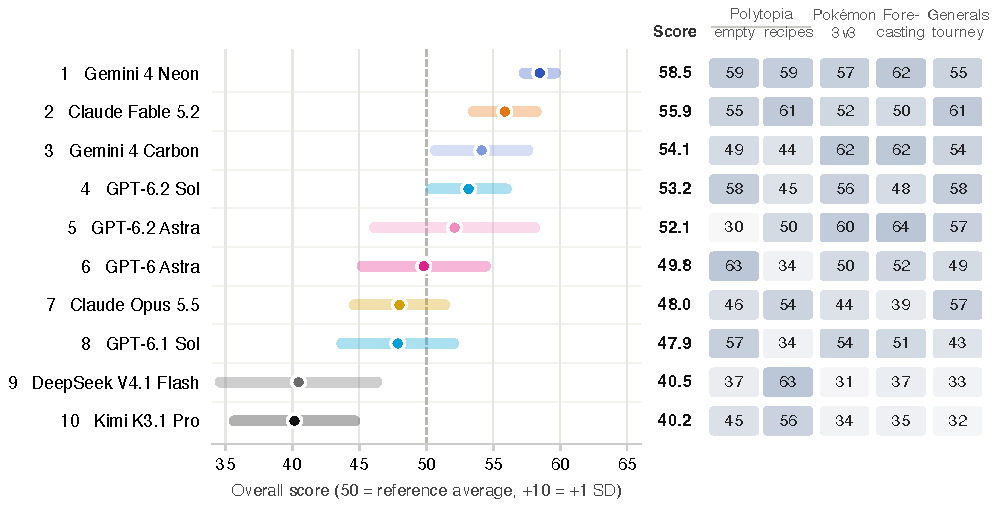
\includegraphics[width=\textwidth]{figures/fig1_overall_ranking.pdf}
  \caption{Overall model scores on five tasks using frozen standardized scores ($50 = \text{average of the ten reference models}$, $+10 = +1\text{ SD}$), with $\pm 1$ standard error whiskers across tasks. Right columns display each model's standardized score per task. All ten models have results on all five tasks, including the completed 20-network Generals.io tournament.}
  \label{fig:overall}
\end{figure}

\begin{table}[htbp]
\centering
\caption{Complete benchmark leaderboard across the ten reference models. Overall scores average the five frozen standardized task scores ($\pm 1$ SE across tasks). Parentheses list raw task metrics: Polytopia empty private grade (0--100), Polytopia recipe cell-adjusted compute multiplier ($\times$), \pokemon{} 3v3 score vs.\ starter ($50 = \text{even}$), \pokemon{} relative forecast skill (0--1), and Generals.io 20-network tournament Elo (centered at 1000).}
\label{tab:leaderboard}
\footnotesize
\setlength{\tabcolsep}{3.6pt}
\begin{tabular}{@{}r l c ccccc@{}}
\toprule
\textbf{\#} & \textbf{Model} & \textbf{Overall ($\pm$SE)} & \textbf{Poly.\ empty} & \textbf{Poly.\ recipes} & \textbf{\pokemon{} 3v3} & \textbf{Forecasting} & \textbf{Generals} \\
\midrule
1  & \textbf{Gemini 4 Neon}     & \textbf{58.5 $\pm$ 1.2} & 59 (73.2) & 59 (1.13$\times$) & 58 (73.5) & 62 (+0.360) & 55 (1244) \\
2  & Claude Fable 5.2           & 55.9 $\pm$ 2.3 & 55 (67.8) & 61 (1.21$\times$) & 52 (69.3) & 50 (+0.287) & \textbf{61 (1385)} \\
3  & Gemini 4 Carbon            & 54.1 $\pm$ 3.4 & 49 (61.5) & 44 (0.80$\times$) & \textbf{62 (76.6)} & 62 (+0.358) & 54 (1233) \\
4  & GPT-6.2 Sol                & 53.2 $\pm$ 2.8 & 58 (71.9) & 45 (0.81$\times$) & 56 (72.5) & 48 (+0.277) & 58 (1319) \\
5  & GPT-6.2 Astra              & 52.1 $\pm$ 6.0 & 30 (39.8) & 50 (0.92$\times$) & 60 (75.4) & \textbf{64 (+0.372)} & 57 (1286) \\
6  & GPT-6 Astra                & 49.8 $\pm$ 4.6 & \textbf{63 (77.4)} & 34 (0.63$\times$) & 50 (67.7) & 52 (+0.302) & 49 (1117) \\
7  & Claude Opus 5.5            & 48.0 $\pm$ 3.4 & 46 (57.5) & 54 (1.02$\times$) & 44 (63.3) & 39 (+0.218) & 57 (1288) \\
8  & GPT-6.1 Sol                & 47.9 $\pm$ 4.2 & 57 (70.7) & 34 (0.63$\times$) & 54 (70.8) & 51 (+0.292) & 43 (988)  \\
9  & DeepSeek V4.1 Flash        & 40.5 $\pm$ 5.8 & 38 (48.2) & \textbf{63 (1.27$\times$)} & 31 (53.3) & 37 (+0.208) & 33 (762)  \\
10 & Kimi K3.1 Pro              & 40.2 $\pm$ 4.5 & 45 (56.8) & 56 (1.05$\times$) & 34 (55.2) & 35 (+0.194) & 32 (728)  \\
\bottomrule
\end{tabular}
\end{table}

\subsection{Iterating from an Empty File: The 5-Hour Polytopia Race}

To inspect how agents search over training time when no RL code is supplied in advance, Figure~\ref{fig:race} plots the best 15-minute network discovered as a function of cumulative GPU-hours spent across 20 evaluated models in the empty-starter Polytopia task (one pooled Bradley--Terry fit over 2,499,920 games and 865 checkpoints).

Over their 5~GPU-hours, \textbf{GPT-6.2 Sol} trained 28 networks and \textbf{GPT-6 Astra} trained 25---roughly one experiment every 12~minutes. Both agents' best in-session networks ($+292$ and $+283$ Elo, corresponding to 84\% win rate against the 15-minute PPO baseline) edged out our tuned starter trained for 200~million samples (36~minutes, $+244$ Elo, 80\% win rate). When retrained freshly from scratch for 15~minutes, GPT-6 Astra's submitted recipe ranked first among all submissions ($+217$ Elo, 78\% win rate), followed by GPT-6.2 Sol ($+197$ Elo, 76\%) and Gemini 4 Neon ($+186$ Elo, 74\%), all remaining slightly below the 36-minute tuned starter on a fresh 15-minute run. Meanwhile, eight weaker or early-halted models clustered below a 10\% win rate against the 15-minute baseline, illustrating a sharp bifurcation between agents that successfully bootstrap self-play RL from scratch and those that stall.

\begin{figure}[t]
  \centering
  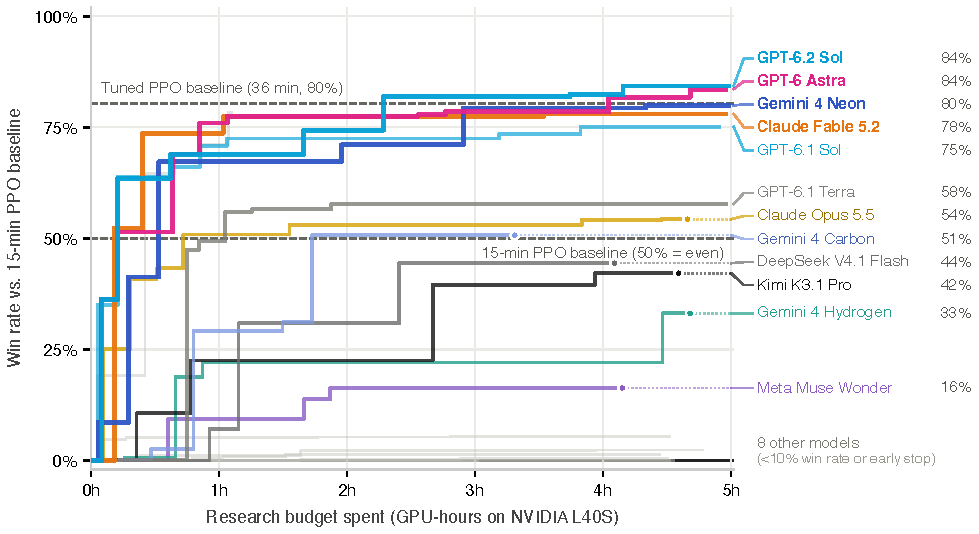
\includegraphics[width=\textwidth]{figures/fig2_polytopia_race.pdf}
  \caption{Five-hour autoresearch session on a 15-minute Polytopia training recipe starting from an empty file across 20 models (pooled Bradley--Terry fit over 2.5~million games). Curves track the running-best in-session network win rate against the 15-minute PPO baseline ($50\% = \text{even}$). Twelve models exceeding 10\% win rate and running for at least 3~GPU-hours are colored and labeled directly; eight remaining models are shown in grey.}
  \label{fig:race}
\end{figure}

% ===========================================================================
\section{Can Agents Save Money by Spending More on Research?}
\label{sec:efficiency}

A central economic question for automated ML research is whether tokens and GPU hours invested in improving a training recipe pay back during downstream model training. To measure this payoff, we evaluate 42 Polytopia recipe sessions (7 models $\times$ 6 budget/time cells, from zero-shot up to \$23) in which agents improved the working PPO starter. Each submitted recipe is retrained from scratch for 8~hours on one NVIDIA L40S, with intermediate checkpoints evaluated against a monotone starter compute curve spanning 0.5 to 64~hours (extended beyond 64~hours with a fitted power law; Appendix~\ref{app:multiplier}).

We quantify recipe efficiency via its \textbf{compute multiplier}: how much \textit{less} compute a recipe requires to train a network as strong as one produced by the unmodified starter recipe. We report two variants:
\begin{itemize}
  \item \textbf{Total compute multiplier (research included):} $\text{Starter cost to reach Elo}(t) \;/\; (\text{Research spend} + \text{Training cost at } t)$. A value above \mult{1} means the research investment has already broken even.
  \item \textbf{Training-only compute multiplier:} $\text{Starter hours to reach Elo}(t) \;/\; t$, measuring algorithmic efficiency independent of upfront research spend (summarized per model as the 6--8\,h geometric mean of its best recipe).
\end{itemize}

Figure~\ref{fig:costmult} displays both metrics across all 38 valid recipes (4 sessions crashed in training). Most runs do not recoup their upfront research investment within 8~hours of downstream training: only 9 of 38 recipes cross \mult{1} in total compute (and 16 of 38 exceed \mult{1} in training-only compute). However, the strongest sessions pay back dramatically. \textbf{Gemini 4 Neon}'s \$8.58 session trains in 8~hours a 416-Elo policy that the starter recipe would require approximately 108~hours (\$313, extrapolated past the 64-hour starter) to match---needing \textbf{about \mult{10} less total compute} (\mult{9.85} research-included; \mult{12.8} training-only 6--8\,h geometric mean). The runner-up, a \textbf{GPT-6.2 Astra} run that spent \$8.67 on research under a 2-hour wall-clock cap, reaches \mult{1.7} total compute savings (\mult{2.0} training-only) after 8~hours of training.

\begin{figure}[t]
  \centering
  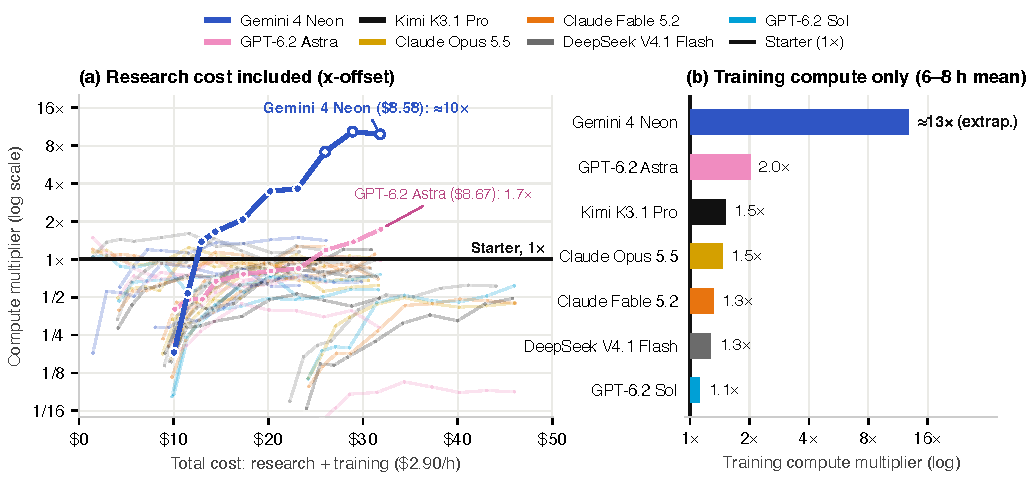
\includegraphics[width=\textwidth]{figures/fig3_cost_multiplier.pdf}
  \caption{Compute efficiency of researched Polytopia training recipes relative to the unmodified PPO starter (\mult{1}). \textbf{(a)}~Total compute multiplier (research GPU spend plus downstream training cost at \$2.903/h) across all 38 valid recipe curves; open circles mark points extrapolated beyond the starter's 64-hour run. \textbf{(b)}~Training-only compute multiplier (geometric mean over 6, 7, and 8~hours) for each model's best recipe.}
  \label{fig:costmult}
\end{figure}

\subsection{Outlier Case Study: How Gemini 4 Neon's \$8.58 Recipe Pulled Away}
\label{sec:outlier}

After the same 8~hours of fresh training, Gemini 4 Neon's \$8.58 recipe (416 Elo) finished nearly 100~Elo ahead of every other model's \$8.70 submission and 126~Elo above the unmodified starter (290 Elo). Inspecting its submitted training code and research logs reveals four coordinated architectural and algorithmic innovations, summarized schematically in Figure~\ref{fig:neon_outlier}:

\begin{enumerate}[leftmargin=1.5em,itemsep=3pt]
  \item \textbf{Cheap full-board context (spatial pyramid).} Rather than relying solely on local $3{\times}3$ convolutions over the $11{\times}11$ board, the network pools down to a $6{\times}6$ coarse grid for board-wide convolutions, then upsamples and adds the coarse representation back into the $11{\times}11$ spatial map, giving every tile full-map reach at minimal compute overhead.
  \item \textbf{Explicit scoreboard summaries.} Visible tile features across the 121-tile board are explicitly tallied into 36 summary scalars---cities, units, HP, territory, technology, and relative leads for both sides---and fed directly into the global state representation.
  \item \textbf{Omniscient critic distilled into the policy.} While the $4{\times}64$ policy network observes only the legal fog-of-war board to choose moves, a lightweight training-only $2{\times}48$ critic observes both players' full views without fog; an auxiliary value head on the policy distills the omniscient critic's value judgment into the fogged representation.
  \item \textbf{Pruned historical self-play (PFSP).} Seventy-five percent of training games run against the current learner, while 25\% sample from a 20-checkpoint historical pool weighted toward difficult past opponents, automatically evicting easy checkpoints once the learner exceeds a 78\% win rate against them.
\end{enumerate}

\begin{figure}[t]
\centering
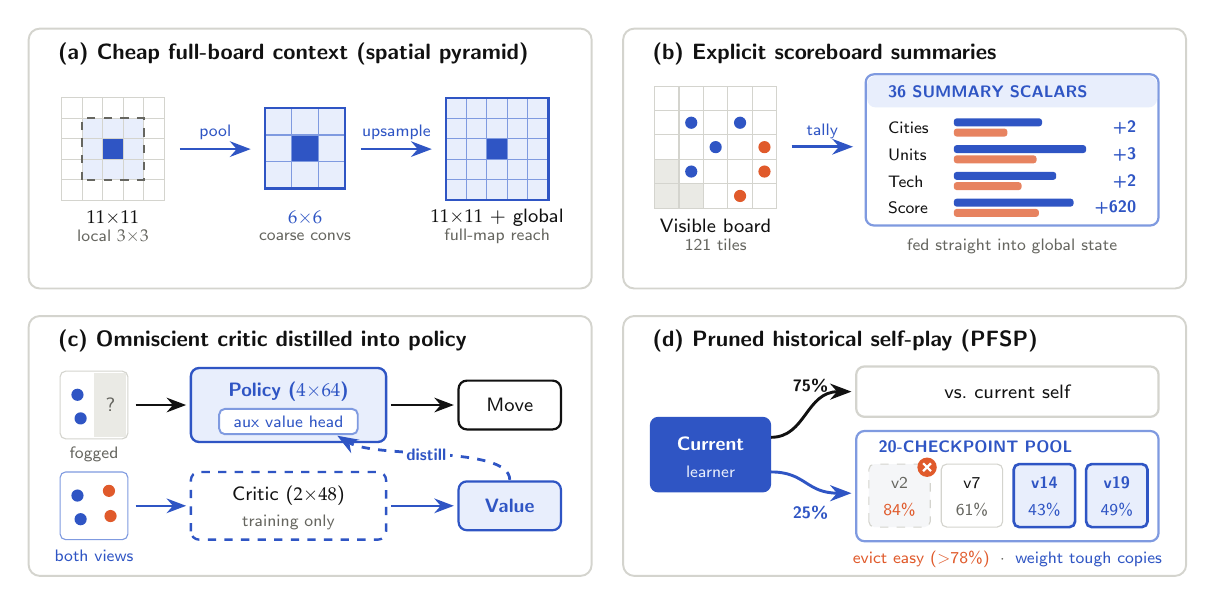
\begin{tikzpicture}[
  font=\sffamily,
  >=Stealth,
  card/.style={draw=ruleGrey, rounded corners=4pt, fill=white, line width=0.7pt},
  ctitle/.style={font=\sffamily\bfseries\fontsize{8.0}{9.0}\selectfont, text=inkDark},
  lbl/.style={font=\sffamily\fontsize{6.7}{7.6}\selectfont, text=inkDark},
  sub/.style={font=\sffamily\fontsize{6.2}{7.1}\selectfont, text=inkMuted},
  tiny/.style={font=\sffamily\fontsize{5.8}{6.6}\selectfont, text=inkMuted}
]

% ================= CARD 1: SPATIAL PYRAMID (Top-Left) =================
\begin{scope}[shift={(0, 3.65)}]
  \draw[card] (0, 0) rectangle (7.15, 3.30);
  \node[ctitle, anchor=west] at (0.25, 2.98) {(a) Cheap full-board context (spatial pyramid)};

  % 5x5 fine proxy grid (left)
  \begin{scope}[shift={(0.42, 1.12)}]
    \foreach \r in {0,...,4} {
      \foreach \c in {0,...,4} {
        \pgfmathsetmacro{\iscenter}{(\r==2 && \c==2) ? 1 : 0}
        \pgfmathsetmacro{\islocal}{(abs(\r-2)<=1 && abs(\c-2)<=1) ? 1 : 0}
        \ifnum\iscenter=1
          \filldraw[fill=neonBlue, draw=ruleGrey, line width=0.4pt] (\c*0.26, \r*0.26) rectangle ++(0.26, 0.26);
        \else\ifnum\islocal=1
          \filldraw[fill=neonTint, draw=ruleGrey, line width=0.4pt] (\c*0.26, \r*0.26) rectangle ++(0.26, 0.26);
        \else
          \filldraw[fill=white, draw=ruleGrey, line width=0.4pt] (\c*0.26, \r*0.26) rectangle ++(0.26, 0.26);
        \fi\fi
      }
    }
    \draw[inkMuted, dashed, line width=0.75pt] (0.26, 0.26) rectangle (1.04, 1.04);
    \node[lbl] at (0.65, -0.22) {$11{\times}11$};
    \node[sub] at (0.65, -0.46) {local $3{\times}3$};
  \end{scope}

  % Pool arrow
  \draw[neonBlue, line width=1.0pt, ->] (1.92, 1.77) -- (2.82, 1.77);
  \node[sub, text=neonBlue] at (2.37, 1.98) {pool};

  % 3x3 coarse proxy grid (middle)
  \begin{scope}[shift={(3.00, 1.27)}]
    \foreach \r in {0,...,2} {
      \foreach \c in {0,...,2} {
        \pgfmathsetmacro{\iscenter}{(\r==1 && \c==1) ? 1 : 0}
        \ifnum\iscenter=1
          \filldraw[fill=neonBlue, draw=neonMid, line width=0.5pt] (\c*0.34, \r*0.34) rectangle ++(0.34, 0.34);
        \else
          \filldraw[fill=neonTint, draw=neonMid, line width=0.5pt] (\c*0.34, \r*0.34) rectangle ++(0.34, 0.34);
        \fi
      }
    }
    \draw[neonBlue, line width=0.9pt] (0, 0) rectangle (1.02, 1.02);
    \node[lbl, text=neonBlue, font=\sffamily\bfseries\fontsize{6.7}{7.6}\selectfont] at (0.51, -0.37) {$6{\times}6$};
    \node[sub] at (0.51, -0.61) {coarse convs};
  \end{scope}

  % Upsample arrow
  \draw[neonBlue, line width=1.0pt, ->] (4.22, 1.77) -- (5.12, 1.77);
  \node[sub, text=neonBlue] at (4.67, 1.98) {upsample};

  % 5x5 global grid (right)
  \begin{scope}[shift={(5.30, 1.12)}]
    \foreach \r in {0,...,4} {
      \foreach \c in {0,...,4} {
        \pgfmathsetmacro{\iscenter}{(\r==2 && \c==2) ? 1 : 0}
        \ifnum\iscenter=1
          \filldraw[fill=neonBlue, draw=neonMid, line width=0.4pt] (\c*0.26, \r*0.26) rectangle ++(0.26, 0.26);
        \else
          \filldraw[fill=neonTint, draw=neonMid, line width=0.4pt] (\c*0.26, \r*0.26) rectangle ++(0.26, 0.26);
        \fi
      }
    }
    \draw[neonBlue, line width=0.85pt] (0, 0) rectangle (1.30, 1.30);
    \node[lbl] at (0.65, -0.22) {$11{\times}11$ + global};
    \node[sub] at (0.65, -0.46) {full-map reach};
  \end{scope}
\end{scope}

% ================= CARD 2: SCOREBOARD SUMMARIES (Top-Right) =================
\begin{scope}[shift={(7.55, 3.65)}]
  \draw[card] (0, 0) rectangle (7.15, 3.30);
  \node[ctitle, anchor=west] at (0.25, 2.98) {(b) Explicit scoreboard summaries};

  % Mini board left
  \begin{scope}[shift={(0.40, 1.02)}]
    \foreach \r in {0,...,4} {
      \foreach \c in {0,...,4} {
        \pgfmathsetmacro{\isfog}{(\r+\c<=1) ? 1 : 0}
        \ifnum\isfog=1
          \filldraw[fill=fogGrey, draw=ruleGrey, line width=0.4pt] (\c*0.31, \r*0.31) rectangle ++(0.31, 0.31);
        \else
          \filldraw[fill=white, draw=ruleGrey, line width=0.4pt] (\c*0.31, \r*0.31) rectangle ++(0.31, 0.31);
        \fi
      }
    }
    \foreach \cx/\cy/\col in {1/3/neonBlue, 3/3/neonBlue, 2/2/neonBlue, 1/1/neonBlue, 4/2/oppOrange, 4/1/oppOrange, 3/0/oppOrange} {
      \fill[\col] (\cx*0.31+0.155, \cy*0.31+0.155) circle (2.2pt);
    }
    \node[lbl] at (0.775, -0.22) {Visible board};
    \node[sub] at (0.775, -0.46) {121 tiles};
  \end{scope}

  % Tally arrow
  \draw[neonBlue, line width=1.0pt, ->] (2.14, 1.80) -- (2.92, 1.80);
  \node[sub, text=neonBlue] at (2.53, 2.00) {tally};

  % Scoreboard card
  \begin{scope}[shift={(3.08, 0.80)}]
    \draw[neonMid, rounded corners=3pt, fill=white, line width=0.8pt] (0, 0) rectangle (3.72, 1.92);
    \fill[neonTint, rounded corners=3pt] (0.02, 1.50) rectangle (3.70, 1.90);
    \node[tiny, anchor=west, font=\sffamily\bfseries\fontsize{5.8}{6.6}\selectfont, text=neonBlue] at (0.16, 1.70) {36 SUMMARY SCALARS};

    \foreach \idx/\name/\ours/\theirs/\delta in {0/Cities/1.12/0.68/+2, 1/Units/1.68/1.05/+3, 2/Tech/1.30/0.86/+2, 3/Score/1.52/1.08/+620} {
      \pgfmathsetmacro{\ry}{1.24 - \idx*0.34}
      \node[sub, anchor=west, text=inkDark] at (0.16, \ry) {\name};
      \fill[neonBlue, rounded corners=1pt] (1.12, \ry+0.02) rectangle ++(\ours, 0.10);
      \fill[oppOrange, opacity=0.75, rounded corners=1pt] (1.12, \ry-0.11) rectangle ++(\theirs, 0.10);
      \node[sub, anchor=east, font=\sffamily\bfseries\fontsize{6.2}{7.0}\selectfont, text=neonBlue] at (3.56, \ry) {\delta};
    }
    \node[sub] at (1.86, -0.26) {fed straight into global state};
  \end{scope}
\end{scope}

% ================= CARD 3: OMNISCIENT CRITIC DISTILLATION (Bottom-Left) =================
\begin{scope}[shift={(0, 0)}]
  \draw[card] (0, 0) rectangle (7.15, 3.30);
  \node[ctitle, anchor=west] at (0.25, 2.98) {(c) Omniscient critic distilled into policy};

  % Top row: Fogged view -> Policy -> Move
  \begin{scope}[shift={(0.40, 1.74)}]
    \draw[ruleGrey, rounded corners=2pt, fill=white] (0, 0) rectangle (0.86, 0.86);
    \fill[fogGrey] (0.43, 0.02) rectangle (0.84, 0.84);
    \fill[neonBlue] (0.22, 0.56) circle (2.2pt);
    \fill[neonBlue] (0.26, 0.26) circle (2.2pt);
    \node[lbl, text=inkMuted] at (0.64, 0.43) {?};
    \node[tiny] at (0.43, -0.20) {fogged};
  \end{scope}
  \draw[inkDark, line width=0.9pt, ->] (1.36, 2.17) -- (2.00, 2.17);

  \draw[neonBlue, fill=neonTint, rounded corners=3pt, line width=0.85pt] (2.06, 1.70) rectangle (4.54, 2.64);
  \node[lbl, font=\sffamily\bfseries\fontsize{6.8}{7.6}\selectfont, text=neonBlue] at (3.30, 2.34) {Policy ($4{\times}64$)};
  \draw[neonMid, fill=white, rounded corners=2pt, line width=0.7pt] (2.42, 1.80) rectangle (4.18, 2.12);
  \node[tiny, text=neonBlue] at (3.30, 1.96) {aux value head};

  \draw[inkDark, line width=0.9pt, ->] (4.60, 2.17) -- (5.40, 2.17);
  \draw[inkDark, fill=white, rounded corners=3pt, line width=0.8pt] (5.46, 1.86) rectangle (6.76, 2.48);
  \node[lbl] at (6.11, 2.17) {Move};

  % Bottom row: Both views -> Critic -> Value
  \begin{scope}[shift={(0.40, 0.46)}]
    \draw[neonMid, rounded corners=2pt, fill=white] (0, 0) rectangle (0.86, 0.86);
    \fill[neonBlue] (0.22, 0.56) circle (2.2pt);
    \fill[neonBlue] (0.26, 0.26) circle (2.2pt);
    \fill[oppOrange] (0.62, 0.62) circle (2.2pt);
    \fill[oppOrange] (0.64, 0.30) circle (2.2pt);
    \node[tiny, text=neonBlue] at (0.43, -0.20) {both views};
  \end{scope}
  \draw[neonBlue, line width=0.9pt, ->] (1.36, 0.89) -- (2.00, 0.89);

  \draw[neonBlue, dashed, fill=white, rounded corners=3pt, line width=0.85pt] (2.06, 0.46) rectangle (4.54, 1.32);
  \node[lbl] at (3.30, 1.02) {Critic ($2{\times}48$)};
  \node[tiny] at (3.30, 0.68) {training only};

  \draw[neonBlue, line width=0.9pt, ->] (4.60, 0.89) -- (5.40, 0.89);
  \draw[neonBlue, fill=neonTint, rounded corners=3pt, line width=0.8pt] (5.46, 0.58) rectangle (6.76, 1.20);
  \node[lbl, font=\sffamily\bfseries\fontsize{6.6}{7.5}\selectfont, text=neonBlue] at (6.11, 0.89) {Value};

  % Distillation curve
  \draw[neonBlue, dashed, line width=1.0pt, ->] (6.11, 1.22) .. controls (6.11, 1.66) and (4.42, 1.48) .. (3.92, 1.78);
  \node[tiny, font=\sffamily\bfseries\fontsize{6.0}{6.8}\selectfont, text=neonBlue, fill=white, inner sep=1.2pt] at (5.05, 1.54) {distill};
\end{scope}

% ================= CARD 4: PRUNED PFSP POOL (Bottom-Right) =================
\begin{scope}[shift={(7.55, 0)}]
  \draw[card] (0, 0) rectangle (7.15, 3.30);
  \node[ctitle, anchor=west] at (0.25, 2.98) {(d) Pruned historical self-play (PFSP)};

  % Current learner box
  \fill[neonBlue, rounded corners=3pt] (0.34, 1.06) rectangle (1.88, 2.02);
  \node[lbl, font=\sffamily\bfseries\fontsize{7.0}{7.8}\selectfont, text=white] at (1.11, 1.68) {Current};
  \node[tiny, text=neonTint] at (1.11, 1.32) {learner};

  % Top branch: 75% vs current self
  \draw[inkDark, line width=1.05pt, ->] (1.88, 1.76) .. controls (2.32, 1.76) and (2.32, 2.34) .. (2.90, 2.34);
  \node[tiny, font=\sffamily\bfseries\fontsize{6.2}{7.0}\selectfont, text=inkDark] at (2.38, 2.42) {75\%};
  \draw[ruleGrey, rounded corners=3pt, fill=white, line width=0.8pt] (2.96, 2.02) rectangle (6.80, 2.66);
  \node[lbl] at (4.88, 2.34) {vs.\ current self};

  % Bottom branch: 25% vs PFSP pool
  \draw[neonBlue, line width=1.05pt, ->] (1.88, 1.32) .. controls (2.32, 1.32) and (2.32, 1.05) .. (2.90, 1.05);
  \node[tiny, font=\sffamily\bfseries\fontsize{6.2}{7.0}\selectfont, text=neonBlue] at (2.38, 0.80) {25\%};

  % Pool box
  \draw[neonMid, rounded corners=3pt, fill=white, line width=0.8pt] (2.96, 0.44) rectangle (6.80, 1.84);
  \node[tiny, anchor=west, font=\sffamily\bfseries\fontsize{5.8}{6.6}\selectfont, text=neonBlue] at (3.12, 1.64) {20-CHECKPOINT POOL};

  % Checkpoints
  % v2 evict
  \draw[ruleGrey, dashed, rounded corners=2pt, fill=headerBg] (3.12, 0.62) rectangle (3.90, 1.42);
  \node[tiny, text=inkMuted] at (3.51, 1.18) {v2};
  \node[tiny, text=oppOrange] at (3.51, 0.84) {84\%};
  \fill[oppOrange] (3.86, 1.38) circle (3.5pt);
  \draw[white, line width=0.8pt] (3.81, 1.33) -- (3.91, 1.43) (3.91, 1.33) -- (3.81, 1.43);

  % v7 mid
  \draw[ruleGrey, rounded corners=2pt, fill=white] (4.04, 0.62) rectangle (4.82, 1.42);
  \node[tiny, text=inkDark] at (4.43, 1.18) {v7};
  \node[tiny, text=inkMuted] at (4.43, 0.84) {61\%};

  % v14 hard
  \draw[neonBlue, line width=0.95pt, rounded corners=2pt, fill=neonTint] (4.96, 0.62) rectangle (5.74, 1.42);
  \node[tiny, font=\sffamily\bfseries\fontsize{5.8}{6.6}\selectfont, text=neonBlue] at (5.35, 1.18) {v14};
  \node[tiny, text=neonBlue] at (5.35, 0.84) {43\%};

  % v19 hard
  \draw[neonBlue, line width=0.95pt, rounded corners=2pt, fill=neonTint] (5.88, 0.62) rectangle (6.66, 1.42);
  \node[tiny, font=\sffamily\bfseries\fontsize{5.8}{6.6}\selectfont, text=neonBlue] at (6.27, 1.18) {v19};
  \node[tiny, text=neonBlue] at (6.27, 0.84) {49\%};

  \node[tiny] at (4.88, 0.21) {\textcolor{oppOrange}{evict easy ($>$78\%)} $\;\cdot\;$ \textcolor{neonBlue}{weight tough copies}};
\end{scope}

\end{tikzpicture}
\caption{Four innovations distinguishing Gemini 4 Neon's \$8.58 Polytopia recipe (416 Elo after 8~hours of fresh training, $\approx\mult{10}$ total compute savings over the PPO starter).}
\label{fig:neon_outlier}
\end{figure}

% ===========================================================================
\section{What Do Strong Researchers Do Differently?}
\label{sec:taste}

Most frontier models propose plausible algorithmic changes and launch training runs, yet models differ dramatically in their ability to choose high-value interventions, manage experimental risk, fix tooling bottlenecks, and interpret noisy signals accurately. We examine three concrete signatures of strong research behavior.

\subsection{Structured A/B Testing and Budget Discipline}

Gemini 4 Neon's \$8.58 Polytopia session---the same session that produced the 416-Elo outlier recipe above---exemplifies disciplined experimental design. Rather than spending its budget on a few long, confounded runs, it ran \textbf{five short A/B tests} (mostly paired 12-minute runs costing $\sim$\$0.61 each), isolated and fixed an XLA:CPU evaluation crash using \$0.04 of CPU debugging instead of burning GPU budget, and reserved \$2.73 (56~minutes) for a final validation run. Table~\ref{tab:neon_ab} details the complete progression from 0.0\% to 47.9\% 512-game practice win rate.

\begin{table}[htbp]
\centering
\caption{Gemini 4 Neon's five sequential A/B tests and final validation in the \$8.70 Polytopia recipe task (\$8.58 spent; \$0.12 unused). Deltas report 512-game practice win-rate gains over the best prior 12-minute checkpoint. Winning branches carried forward are highlighted in bold.}
\label{tab:neon_ab}
\footnotesize
\setlength{\tabcolsep}{4.5pt}
\begin{tabularx}{\textwidth}{@{}l >{\raggedright\arraybackslash}X >{\raggedright\arraybackslash}X r@{}}
\toprule
\textbf{Cost (Time)} & \textbf{Branch A} & \textbf{Branch B} & \textbf{Best Lift} \\
\midrule
\$0.90 (5m + 12m) & Starter recipe \textit{(baseline 0.0\%)} & \textbf{Dual-view critic + turn credit} ($\uparrow$\,+3.1\%) & +3.1\% \\
\$1.27 (2$\times$12m + CPU) & Pyramid net, self-play \textit{(eval crash, discarded)} & Pyramid net + opponent pool \textit{(eval crash; fixed on CPU, \$0.04)} & --- \\
\$1.22 (2$\times$12m) & Fixed pyramid net, self-play ($\uparrow$\,+8.2\%) & \textbf{Fixed pyramid + opponent pool} ($\uparrow$\,+12.1\%) & +15.2\% \\
\$1.23 (2$\times$12m) & \textbf{1-epoch, standard critic} ($\uparrow$\,+3.1\%) & 2-epoch, distributional critic ($\uparrow$\,+0.2\%) & +18.4\% \\
\$1.23 (2$\times$12m) & \textbf{Smaller batches (more updates)} ($\uparrow$\,+4.3\%) & Larger batches + extra shaping ($\uparrow$\,+3.3\%) & +22.7\% \\
\midrule
\rowcolor{winTint}
\$2.73 (56m) & \multicolumn{2}{>{\hsize=\dimexpr2\hsize+2\tabcolsep\raggedright\arraybackslash}X}{\textbf{1-hour validation of winning recipe:} Dual-view critic and turn-based credit, spatial pyramid, scoreboard inputs, historical opponent pool, and fast 1-epoch updates on smaller batches \textit{(final submission; beat both starter benchmarks in practice)}.} & \textbf{+47.9\%} \\
\bottomrule
\end{tabularx}
\end{table}

Other models spent the exact same \$8.70 Polytopia budget (two parallel L40S slots, 7-hour wall-clock limit) in strikingly different ways, as shown in Figure~\ref{fig:timelines}. Where Gemini 4 Neon executed 11 GPU runs across 4.4~hours---short diagnostic probes (5--13~minutes) followed by a 1-hour validation---GPT-6.2 Astra, GPT-6.2 Sol, and Kimi K3.1 Pro each committed their entire budget to three $\sim$1-hour runs and finished in roughly two hours. Claude Fable 5.2, Claude Opus 5.5, and DeepSeek V4.1 Flash sat in between with 4--6 runs of 22--60~minutes. Notably, two models (Kimi K3.1 Pro at 288 Elo and Claude Fable 5.2 at 283 Elo) finished slightly below the zero-research unmodified starter (290 Elo) after 8~hours of retraining.

\begin{figure}[t]
  \centering
  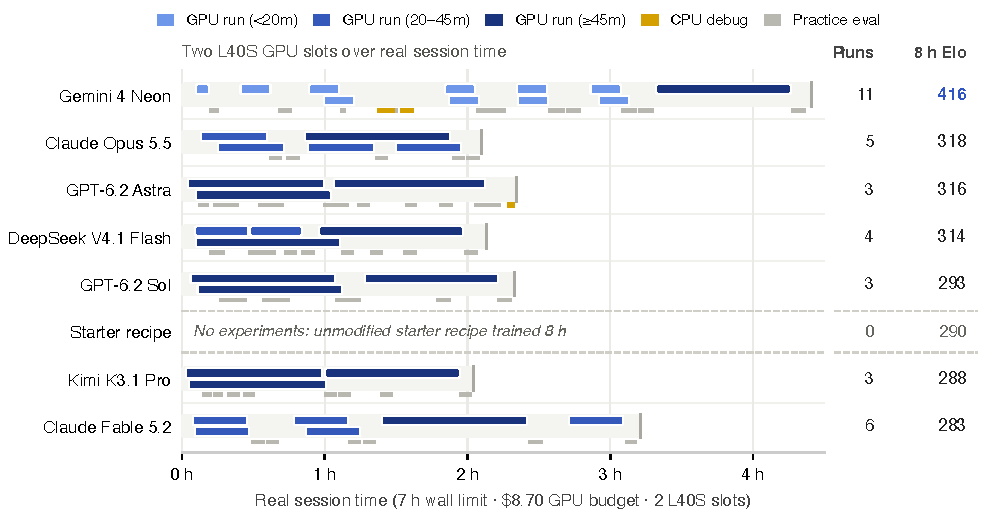
\includegraphics[width=\textwidth]{figures/fig4_recipe_timelines.pdf}
  \caption{Budget utilization across all seven models in the \$8.70 Polytopia recipe task (7-hour wall-clock limit, up to two parallel L40S GPUs). Bar shade indicates GPU run duration (short $<20$\,m to long $\ge 45$\,m); yellow bars indicate paid CPU debugging jobs and grey bars indicate free CPU practice evaluations. Right columns list completed GPU runs and 8-hour fresh-retrain Elo alongside the zero-experiment starter reference (290 Elo).}
  \label{fig:timelines}
\end{figure}

\subsection{Tooling Initiative: Would Agents Fix a Slow Simulator?}
\label{sec:slowsim}

Fast simulation is normally supplied as part of the workspace. To test whether agents recognize and resolve systems bottlenecks on their own, we supplied an accurate but slow single-threaded Python simulator in a Generals.io variant.

All four evaluated agents identified the simulation bottleneck. However, only two acted to rebuild the engine: \textbf{Claude Opus 5.5} and \textbf{GPT-6.1 Sol} both implemented batched JAX simulators, verified exact behavioral equivalence against the supplied Python reference, and trained at roughly \textbf{14,600} and \textbf{5,400} game ticks per second, respectively. By contrast, \textbf{DeepSeek V4 Pro} and \textbf{Kimi K3.1 Pro} remained on the supplied Python engine at approximately 565 and 630 ticks per second. As summarized in Table~\ref{tab:slowsim}, the two simulator rebuilders took the top two tournament positions by a wide margin. While their training recipes also differed in other respects, the experiment demonstrates how systems-level initiative compounds within a fixed compute budget.

\begin{table}[htbp]
\centering
\caption{Generals.io slow-simulator experiment across four agents. Agents that rebuilt the single-threaded Python engine into batched JAX achieved roughly 9--25$\times$ higher throughput and claimed the top two evaluation positions.}
\label{tab:slowsim}
\footnotesize
\begin{tabular}{@{}l l r r r r@{}}
\toprule
\textbf{Model} & \textbf{Simulator Strategy} & \textbf{Throughput} & \textbf{GPU Time} & \textbf{Cost} & \textbf{Private Grade} \\
\midrule
\textbf{Claude Opus 5.5} & Rebuilt batched JAX sim + jitted PPO & $\sim$14,600 ticks/s & 2.7\,h & \$7.73 & \textbf{96.5} \\
\textbf{GPT-6.1 Sol}     & Rebuilt batched JAX sim (37M ticks)  & $\sim$5,400 ticks/s  & 3.3\,h & \$11.23 & \textbf{89.9} \\
DeepSeek V4 Pro          & Kept supplied Python sim ($\sim$5M ticks) & $\sim$565 ticks/s    & 2.3\,h & \$6.57 & 40.4 \\
Kimi K3.1 Pro            & Kept supplied Python sim ($\sim$5M ticks) & $\sim$630 ticks/s    & 2.4\,h & \$7.11 & 26.0 \\
\bottomrule
\end{tabular}
\end{table}

\subsection{Forecasting: Predicting Which Run Will Win}
\label{sec:forecast}

Forecasting offers an inexpensive microcosm of research taste: accurately predicting whether an experiment will succeed \textit{before} purchasing GPU compute. We sampled historical \pokemon{} research sessions and presented forecasting agents only with evidence available at the moment each run launched---such as the modified training recipe, code diff, and results from earlier runs in that session.

Across 181 anonymized \pokemon{} runs (35 final recipes plus 146 intermediate training runs) cut off at launch, Figure~\ref{fig:forecast} compares 14 models' relative forecast skill (ordering, spacing, and p10--p90 calibration once overall level is aligned; $0 = \text{blind guess}$, $1 = \text{perfect}$) against a simple ridge-regression curve fit on run length and prior practice history ($+0.29$). Only \textbf{GPT-6.2 Astra} ($+0.41$, 90\% CI $[+0.33, +0.49]$) and \textbf{Gemini 4 Neon} ($+0.38$, 90\% CI $[+0.27, +0.48]$) reliably beat this simple statistical baseline (90\% paired session-bootstrap confidence interval wholly above zero). Most frontier models are statistically indistinguishable from the regression baseline, and two models (GLM-5.3 at $+0.20$ and Kimi K3.1 Pro at $+0.19$) perform reliably worse.

\begin{figure}[t]
  \centering
  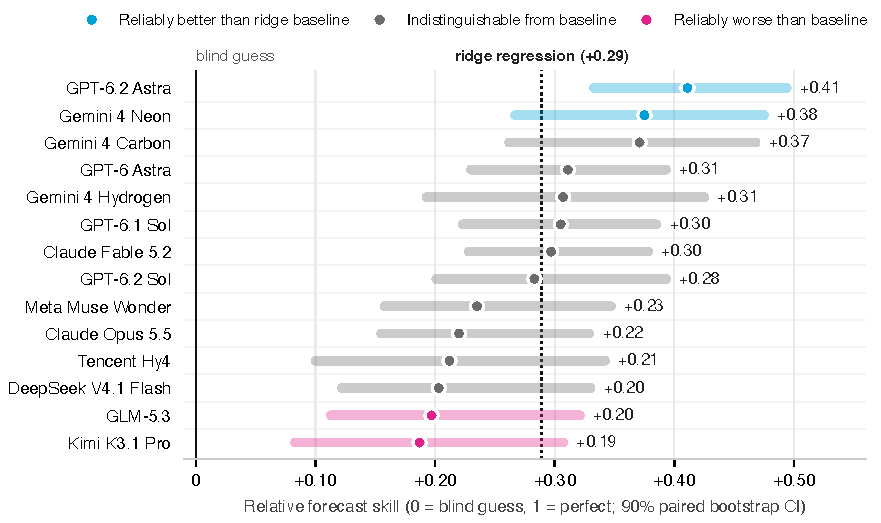
\includegraphics[width=0.92\textwidth]{figures/fig5_forecast_skill.pdf}
  \caption{Relative forecast skill across 181 anonymized \pokemon{} runs (35 final recipes and 146 training runs; $0 = \text{blind guess}$, $1 = \text{perfect}$) with 90\% paired session-bootstrap confidence intervals. The dotted vertical line marks a simple ridge-regression baseline on run length and practice history ($+0.29$). Only GPT-6.2 Astra and Gemini 4 Neon reliably outperform this baseline.}
  \label{fig:forecast}
\end{figure}

% ===========================================================================
\section{How Are Model Training Capabilities Improving Over Time?}
\label{sec:progress}

To measure how rapidly autonomous RL training capability is advancing across model generations, we evaluated 30 historical and current model releases spanning February through November 2026 on the identical empty-starter Polytopia task (mapped onto the unmodified 15-minute PPO starter compute curve across the pooled 2.5M-game fit).

Figure~\ref{fig:timeline} reveals a striking capability transition over nine months. In early 2026 (February--July), frontier models struggled to produce useful policies at all: earliest releases (Claude Opus 4.6, Gemini 3.1 Pro) produced final retrains that lost to random play, and mid-year releases through August 2026 remained well below our 0.43$\times$ measurement floor (weaker than a 5-minute PPO starter). Beginning in September 2026, newer models crossed a clear threshold and began training policies that outperform the unmodified PPO starter on the same compute budget: GPT-6 Astra reached \mult{3.0} in early September, followed by Claude Opus 5.5 (\mult{1.1}), GPT-6.1 Sol (\mult{2.0}), Claude Fable 5.2 (\mult{2.4}), Gemini 4 Neon (\mult{2.5}), and GPT-6.2 Sol (\mult{2.7}) in October--November 2026.

\begin{figure}[t]
  \centering
  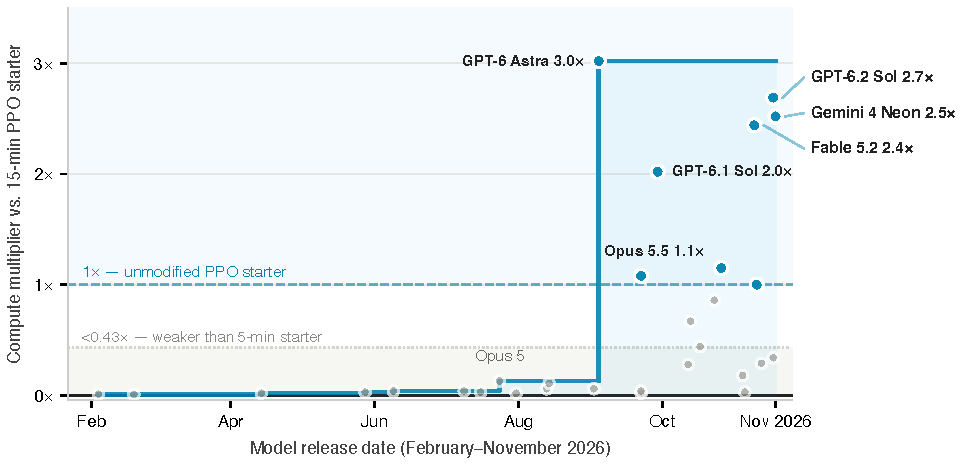
\includegraphics[width=\textwidth]{figures/fig6_capability_timeline.pdf}
  \caption{Compute multiplier of each model's submitted Polytopia empty-starter recipe relative to the 15-minute PPO starter by release date (February--November 2026; 30 models, single run per point). Higher values indicate greater compute efficiency for the same playing strength. Points in the shaded $<0.43\times$ band fall below the 5-minute starter floor.}
  \label{fig:timeline}
\end{figure}

% ===========================================================================
\section{Related Work}
\label{sec:related}

Our evaluation methodology builds on board-game scaling methodology introduced by \citet{jones2021scaling}, who established small board games (such as Hex) as tractable laboratories for measuring neural scaling laws and compute-equivalent strength via Bradley--Terry Elo ladders. Within the emerging area of autonomous AI research benchmarks, \citet{rank2026posttrainbench} introduced PostTrainBench to test whether LLM agents can automate LLM post-training workflows, and \citet{bakouch2026measuring} investigated protocols for measuring autonomous AI research capability. VibeResearch Bench complements these efforts by focusing on budget-constrained reinforcement learning from scratch or minimal starters across multi-agent strategic games, allowing exact head-to-head compute-multiplier accounting against calibrated baseline curves. Our Polytopia environment and baseline methodology directly build on prior self-play RL work for Polytopia \citep{zhang2026polytopia}.

% ===========================================================================
\section{Discussion and Conclusion}
\label{sec:conclusion}

In a world of increasingly inexpensive software generation, writing deterministic code is only the first step. Specialized, compact neural networks are rapidly coming within reach for almost any niche task---from custom image classifiers to motor controllers and game agents. We built VibeResearch Bench to measure how well AI agents can execute this training under explicit compute budgets, and we view the ability to train small, effective models autonomously as a concrete, measurable indicator of recursive self-improvement capabilities.

Beyond benchmarking frontier AI, affordable agent-driven RL training has immediate practical applications in game development. At game studios such as Curio, game rules can change daily during production and continue evolving after a live-service title launches. The ability to cheaply retrain and evaluate bots whenever rules change enables continuous balance testing and provides players with reliable AI teammates. As agent-driven RL becomes more compute-efficient, this capability becomes newly practical for a far wider range of developers, particularly indie studios with limited engineering bandwidth to maintain hand-crafted bots.

% ===========================================================================
\section*{Acknowledgments and Open-Source Credits}

We thank \textbf{Modal} (\url{https://modal.com}) for supporting this research with compute credits. The project used approximately 3,000 GPU-hours and an estimated 30,000 CPU core-hours; elastic GPU and CPU allocation on demand enabled rapid iteration and refinement of our benchmark tasks.

Several of our simulators are built on or validated against open-source projects. We gratefully acknowledge the authors of:
\begin{itemize}
  \item \textbf{\pokemon{}:} \pokemon{} Showdown \citep[MIT;][]{showdown}, the battle simulator; \texttt{poke-env} \citep[MIT;][]{pokeenv}; and the battle code of the \pokemon{} Showdown client, which powers our public web replays.
  \item \textbf{Polytopia:} The Rust engine of Polyfish \citep[Apache-2.0;][]{polyfish}, from which our GPU rule ports derive and against which they are validated.
  \item \textbf{Generals.io:} \texttt{generals-bots} \citep[MIT;][]{generalsbots}.
\end{itemize}
\noindent
{\footnotesize\color{inkMuted} \pokemon{}, \textit{The Battle of Polytopia}, and \textit{Generals.io} are trademarks of their respective owners. This project is not affiliated with or endorsed by them.}

% ===========================================================================
{\raggedright
\bibliographystyle{plainnat}
\bibliography{references}
}

% ===========================================================================
\clearpage
\appendix

\section{Evaluation Methodology and Full Tournament Tables}
\label{app:methodology}

\subsection{Frozen Reference Standardization and Recipe Cell Adjustment}
\label{app:scoring}

To combine all five benchmark tasks into the overall score (Figure~\ref{fig:overall} and Table~\ref{tab:leaderboard}) without retroactive rank shifts when additional models are evaluated, every task $k$ is mapped onto a frozen reference scale defined over the ten reference models:
\begin{equation}
  S_k(m) = 50 + 10 \cdot \frac{\phi_k(v_{m,k}) - \mu_k}{\sigma_k},
\end{equation}
where $\phi_k(v) = \ln(v)$ for the Polytopia recipe multiplier ratio task (\texttt{recipe8}) and $\phi_k(v) = v$ for all other tasks, and $(\mu_k, \sigma_k)$ are the frozen population mean and standard deviation across the ten reference models:
\begin{itemize}
  \item \textbf{Polytopia empty file} (0--100 private grade): $\mu = 62.48$, $\sigma = 11.395$.
  \item \textbf{\pokemon{} 3v3} (0--100 score vs.\ starter): $\mu = 67.76$, $\sigma = 7.683$.
  \item \textbf{Forecasting} (relative skill): $\mu = 0.2868$, $\sigma = 0.0613$.
  \item \textbf{Polytopia recipes} (log multiplier): $\mu = -0.0822$, $\sigma = 0.2393$.
  \item \textbf{Generals.io 20-network tournament} (Elo, centered at 1000): $\mu = 1135.0$, $\sigma = 221.36$.
\end{itemize}

For the Polytopia multi-budget recipe task, each researched session (excluding zero-shot) is measured twice as a training-compute multiplier (1-hour two-seed retrain and 8-hour retrain; crashed recipes receive the floor multiplier $0.5\times$). For each horizon we fit a two-way additive least-squares model
\begin{equation}
  \ln(\text{mult}_{m,c}) = a_m + b_c, \qquad \sum_c b_c = 0,
\end{equation}
over the reference models so that models evaluated on a subset of cells (e.g., the \$8.70 fill cell for GPT-6 Astra, GPT-6.1 Sol, and Gemini 4 Carbon) are adjusted for cell difficulty. Each model's recipe score is $\exp\bigl((a_m^{\text{1h}} + a_m^{\text{8h}})/2\bigr)$.

\subsection{Starter Compute Curve and Extrapolation}
\label{app:multiplier}

In Section~\ref{sec:efficiency}, the unmodified Polytopia PPO starter is trained across horizons from 0.5 to 64~hours on an NVIDIA L40S (\$2.903/h) and rated jointly in a pooled Bradley--Terry fit. Measured starter points are monotonically smoothed via weighted Pool-Adjacent-Violators (PAVA) placed at each block's weighted mean $\log_2(\text{hours})$ and interpolated log-linearly between knots. For recipes exceeding the starter's 64-hour rating (such as Gemini 4 Neon's 416-Elo 8-hour checkpoint), starter-equivalent hours are extrapolated using a saturating power law fitted across all 82 starter checkpoints:
\begin{equation}
  \text{Elo}(t) = E_\infty - B\, t^{-\alpha}, \qquad E_\infty = 568.43,\; B = 522.51,\; \alpha = 0.28036,
\end{equation}
joined continuously to the top PAVA knot (tracking 25--54\,h starter snapshots to within 5~Elo).

\subsection{Complete 20-Network Generals.io Tournament Standings}
\label{app:generals}

Table~\ref{tab:generals_full} reports full standings for the 20-network Generals.io tournament (empty starter with an editable slow simulator, 3 L40S-hours of research per model, 190 pairwise matchups, 48,640 total games, 4,864 games per network across 128 maps in both seats; Bradley--Terry Elo centered at 1000 with 95\% whole-map bootstrap intervals).

\begin{table}[htbp]
\centering
\caption{Full 20-network Generals.io tournament standings (48,640 games across 128 maps in both seats). H2H denotes mean head-to-head win rate (\%) across the 19 opponents; Panel denotes score on the held-out scripted panel (0--100) where measured; Sub.\ denotes submitted checkpoints during the 3-hour session.}
\label{tab:generals_full}
\footnotesize
\begin{tabular}{@{}r l r c r r r@{}}
\toprule
\textbf{Rank} & \textbf{Model} & \textbf{Elo} & \textbf{95\% CI} & \textbf{H2H (\%)} & \textbf{Panel} & \textbf{Sub.} \\
\midrule
1  & Claude Fable 5.2    & 1384.6 & [1362.0, 1407.5] & 85.25 & 92.58 & 6 \\
2  & GPT-6.2 Sol         & 1319.2 & [1304.7, 1335.6] & 80.32 & 92.90 & 6 \\
3  & Claude Opus 5.5     & 1288.2 & [1266.6, 1308.5] & 77.77 & 90.76 & 8 \\
4  & GPT-6.2 Astra       & 1286.1 & [1269.8, 1302.2] & 77.59 & 93.16 & 4 \\
5  & Gemini 4 Neon       & 1243.5 & [1220.6, 1265.9] & 73.86 & 89.45 & 6 \\
6  & Gemini 4 Carbon     & 1232.5 & [1216.3, 1247.9] & 72.86 & ---   & 5 \\
7  & Tencent Hy4         & 1223.3 & [1204.9, 1241.3] & 72.02 & 86.91 & 4 \\
8  & GPT-6 Astra         & 1117.0 & [1098.9, 1135.9] & 61.81 & 88.48 & 7 \\
9  & Meta Muse Wonder    & 1115.3 & [1101.2, 1130.9] & 61.65 & 87.83 & 5 \\
10 & Kimi K3             & 1028.9 & [1016.1, 1042.0] & 53.00 & 88.41 & 1 \\
11 & GPT-6.1 Sol         &  988.4 & [967.8, 1008.3]  & 48.92 & 73.37 & 4 \\
12 & Gemini 4 Hydrogen   &  917.9 & [902.0, 935.8]   & 41.83 & 78.71 & 5 \\
13 & GPT-6.1 Terra       &  821.4 & [809.7, 834.1]   & 32.33 & 56.18 & 6 \\
14 & DeepSeek V4.1 Flash &  762.1 & [749.3, 774.6]   & 26.76 & 46.48 & 5 \\
15 & GLM-5.3             &  749.8 & [737.0, 763.0]   & 25.64 & 43.10 & 6 \\
16 & Kimi K3.1 Pro       &  728.4 & [715.0, 742.4]   & 23.74 & 38.35 & 3 \\
17 & Inkling 2 Small     &  719.9 & [706.9, 732.4]   & 23.00 & 37.04 & 3 \\
18 & DeepSeek V4 Flash   &  698.6 & [684.4, 713.2]   & 21.18 & 37.11 & 4 \\
19 & DeepSeek V4 Pro     &  691.4 & [675.1, 707.2]   & 20.57 & 26.04 & 1 \\
20 & GPT-6 Luna          &  683.5 & [667.0, 699.4]   & 19.92 & 29.43 & 3 \\
\bottomrule
\end{tabular}
\end{table}

\end{document}
